% Options for packages loaded elsewhere
\PassOptionsToPackage{unicode}{hyperref}
\PassOptionsToPackage{hyphens}{url}
%
\documentclass[
]{article}
\usepackage{lmodern}
\usepackage{amssymb,amsmath}
\usepackage{ifxetex,ifluatex}
\ifnum 0\ifxetex 1\fi\ifluatex 1\fi=0 % if pdftex
  \usepackage[T1]{fontenc}
  \usepackage[utf8]{inputenc}
  \usepackage{textcomp} % provide euro and other symbols
\else % if luatex or xetex
  \usepackage{unicode-math}
  \defaultfontfeatures{Scale=MatchLowercase}
  \defaultfontfeatures[\rmfamily]{Ligatures=TeX,Scale=1}
\fi
% Use upquote if available, for straight quotes in verbatim environments
\IfFileExists{upquote.sty}{\usepackage{upquote}}{}
\IfFileExists{microtype.sty}{% use microtype if available
  \usepackage[]{microtype}
  \UseMicrotypeSet[protrusion]{basicmath} % disable protrusion for tt fonts
}{}
\makeatletter
\@ifundefined{KOMAClassName}{% if non-KOMA class
  \IfFileExists{parskip.sty}{%
    \usepackage{parskip}
  }{% else
    \setlength{\parindent}{0pt}
    \setlength{\parskip}{6pt plus 2pt minus 1pt}}
}{% if KOMA class
  \KOMAoptions{parskip=half}}
\makeatother
\usepackage{xcolor}
\IfFileExists{xurl.sty}{\usepackage{xurl}}{} % add URL line breaks if available
\IfFileExists{bookmark.sty}{\usepackage{bookmark}}{\usepackage{hyperref}}
\hypersetup{
  pdftitle={Project 1 Report},
  pdfauthor={Alexandre Lockhart},
  hidelinks,
  pdfcreator={LaTeX via pandoc}}
\urlstyle{same} % disable monospaced font for URLs
\usepackage[margin=1in]{geometry}
\usepackage{color}
\usepackage{fancyvrb}
\newcommand{\VerbBar}{|}
\newcommand{\VERB}{\Verb[commandchars=\\\{\}]}
\DefineVerbatimEnvironment{Highlighting}{Verbatim}{commandchars=\\\{\}}
% Add ',fontsize=\small' for more characters per line
\usepackage{framed}
\definecolor{shadecolor}{RGB}{248,248,248}
\newenvironment{Shaded}{\begin{snugshade}}{\end{snugshade}}
\newcommand{\AlertTok}[1]{\textcolor[rgb]{0.94,0.16,0.16}{#1}}
\newcommand{\AnnotationTok}[1]{\textcolor[rgb]{0.56,0.35,0.01}{\textbf{\textit{#1}}}}
\newcommand{\AttributeTok}[1]{\textcolor[rgb]{0.77,0.63,0.00}{#1}}
\newcommand{\BaseNTok}[1]{\textcolor[rgb]{0.00,0.00,0.81}{#1}}
\newcommand{\BuiltInTok}[1]{#1}
\newcommand{\CharTok}[1]{\textcolor[rgb]{0.31,0.60,0.02}{#1}}
\newcommand{\CommentTok}[1]{\textcolor[rgb]{0.56,0.35,0.01}{\textit{#1}}}
\newcommand{\CommentVarTok}[1]{\textcolor[rgb]{0.56,0.35,0.01}{\textbf{\textit{#1}}}}
\newcommand{\ConstantTok}[1]{\textcolor[rgb]{0.00,0.00,0.00}{#1}}
\newcommand{\ControlFlowTok}[1]{\textcolor[rgb]{0.13,0.29,0.53}{\textbf{#1}}}
\newcommand{\DataTypeTok}[1]{\textcolor[rgb]{0.13,0.29,0.53}{#1}}
\newcommand{\DecValTok}[1]{\textcolor[rgb]{0.00,0.00,0.81}{#1}}
\newcommand{\DocumentationTok}[1]{\textcolor[rgb]{0.56,0.35,0.01}{\textbf{\textit{#1}}}}
\newcommand{\ErrorTok}[1]{\textcolor[rgb]{0.64,0.00,0.00}{\textbf{#1}}}
\newcommand{\ExtensionTok}[1]{#1}
\newcommand{\FloatTok}[1]{\textcolor[rgb]{0.00,0.00,0.81}{#1}}
\newcommand{\FunctionTok}[1]{\textcolor[rgb]{0.00,0.00,0.00}{#1}}
\newcommand{\ImportTok}[1]{#1}
\newcommand{\InformationTok}[1]{\textcolor[rgb]{0.56,0.35,0.01}{\textbf{\textit{#1}}}}
\newcommand{\KeywordTok}[1]{\textcolor[rgb]{0.13,0.29,0.53}{\textbf{#1}}}
\newcommand{\NormalTok}[1]{#1}
\newcommand{\OperatorTok}[1]{\textcolor[rgb]{0.81,0.36,0.00}{\textbf{#1}}}
\newcommand{\OtherTok}[1]{\textcolor[rgb]{0.56,0.35,0.01}{#1}}
\newcommand{\PreprocessorTok}[1]{\textcolor[rgb]{0.56,0.35,0.01}{\textit{#1}}}
\newcommand{\RegionMarkerTok}[1]{#1}
\newcommand{\SpecialCharTok}[1]{\textcolor[rgb]{0.00,0.00,0.00}{#1}}
\newcommand{\SpecialStringTok}[1]{\textcolor[rgb]{0.31,0.60,0.02}{#1}}
\newcommand{\StringTok}[1]{\textcolor[rgb]{0.31,0.60,0.02}{#1}}
\newcommand{\VariableTok}[1]{\textcolor[rgb]{0.00,0.00,0.00}{#1}}
\newcommand{\VerbatimStringTok}[1]{\textcolor[rgb]{0.31,0.60,0.02}{#1}}
\newcommand{\WarningTok}[1]{\textcolor[rgb]{0.56,0.35,0.01}{\textbf{\textit{#1}}}}
\usepackage{graphicx,grffile}
\makeatletter
\def\maxwidth{\ifdim\Gin@nat@width>\linewidth\linewidth\else\Gin@nat@width\fi}
\def\maxheight{\ifdim\Gin@nat@height>\textheight\textheight\else\Gin@nat@height\fi}
\makeatother
% Scale images if necessary, so that they will not overflow the page
% margins by default, and it is still possible to overwrite the defaults
% using explicit options in \includegraphics[width, height, ...]{}
\setkeys{Gin}{width=\maxwidth,height=\maxheight,keepaspectratio}
% Set default figure placement to htbp
\makeatletter
\def\fps@figure{htbp}
\makeatother
\setlength{\emergencystretch}{3em} % prevent overfull lines
\providecommand{\tightlist}{%
  \setlength{\itemsep}{0pt}\setlength{\parskip}{0pt}}
\setcounter{secnumdepth}{-\maxdimen} % remove section numbering
\usepackage{booktabs}
\usepackage{longtable}
\usepackage{array}
\usepackage{multirow}
\usepackage{wrapfig}
\usepackage{float}
\usepackage{colortbl}
\usepackage{pdflscape}
\usepackage{tabu}
\usepackage{threeparttable}
\usepackage{threeparttablex}
\usepackage[normalem]{ulem}
\usepackage{makecell}

\title{Project 1 Report}
\author{Alexandre Lockhart}
\date{10/14/2020}

\begin{document}
\maketitle

\hypertarget{overall-objectives}{%
\subsection{Overall objectives}\label{overall-objectives}}

The war of correlates projects curates war data from 1814 globally
through 2014 from all around the world. Variables such as deaths,
outcome status, perceived initiator, periods of exposure, forces
involved, whether the war was internationalized and spread and many
other variables have been collected. Additional datasets such as
economic factors, etc. have also been collected and tabulated with
multiple datasets but the previously mentioned variables were of main
interest for this project.

Due to the time period of curation (1814-2014), and the onset of the
Monroe Doctrine in 1823, the central interest in this project was to
look at the role of Americas (or the US and South America) versus the
rest of the world in initiator-defined outcomes. This was historic in
that in set a role of the United States in dictating colonial policy
within the hemisphere up as north of Canada through the southern tip of
Latin America in order to mandate control and keep international powers
at bay cementing a power structure that has lasted until modern 21st
century. The word initiator is used a lot in this project and is defined
as the perceived initial war aggressor. Recipient is the perceived
country who is the recipient of the initiator's attack.

Initially the project involved looking at initial descriptive
relationships of the Americas versus non-Americas conflict via tables
and graphs in the domestic wars only dataset. Variables such as deaths,
type of conflict, internationalization of conflict, the Americas
indicator of interest, exposure time of given conflict, and initiator
created variables such as the absolute difference in initiator versus
recipient deaths, and relative difference in the initiator to recipient
deaths were visually examined.

Aim 1 of the project involved looking at Americas versus non-Americas in
initiator determined outcomes such as: absolute difference in initiator
versus recipient deaths and relative difference in initiator versus
recipient deaths, . Initial basic glm models would be assessed while
including war type, start year, and number of days of exposure. This
would be repeated for the absolute and relative difference outcomes and
then repeated using a training and testing set to assess prediction. The
sensitivity of prediction would be assessed via imputation of deaths
where missing, recomputing absolute and relative initiator variables of
interest, and re-doing the prediction models.. The entire process would
be repeated on an internationalized dataset, or one which adds forces
available to those in conflict as well as adds additional wars perceived
to be linked to the initial model set on an international scale.

Aim 2 was multi-fold: to cluster wartype, the Americas indicator
variable, time since war started since 1814 basically, whether the war
was internationalized, duration of exposure (days), initiator deaths,
recipient deaths, and relative difference in deaths via a distance
metric for mixed data types. Besides cluster assessment and performance
evaluation, the clusters were then descriptively assessed with
clustering variables as well as the conflict outcome for pattern
assessment.\\

The final aim 3 was to look at network community detection based on
weighting relative difference in deaths. A network data structure was
made utilizing these weights. The goal was to descriptively assign
membership and look at potentially separating attributes for a given
community membership.

\#Preprocessing Type of war was consolidated to Civil War: Central
Control, Civil War: Local issues, and then other to account for sparsity
of the last two categories. It is important to know that an
internationalized dataset is also used (not shown) which adds wars to
relevant wars that had conflict extend outside their local boundaries
and also included forces available for each side in the conflict.

Initiator/recipient deaths and then the final outcome (`outcome E') was
created by an indicator of initiator in the dataset as well as variables
for side A/side B deaths and pattern matching in their construction.
Imputations of the initiator and recipient death variables were created
to account for missingness and eventual sensitivity analyses in
prediction.

Test.An initial table 1 is shown below of demographics by the Americas
and non-Americas indicator variable of main interest in the project. Not
surprisingly, the number of regions and countries, etc. are going to
have more wars representing 5/7 countries in the `Not in Americas'
category. Among the Americas, the distribution of wars classified as
central control dominated proportionally (81\%) while the war types were
more balances in the not in Americas group. While the variability was
high, the mean total days of war in the Americas versus Not in Americas
was over 124 days less. Absolute difference in deaths
(Initiator-recipient deaths) showed a much higher liability towards the
initiator among conflicts in the Americas relative to Not in Americas.
The time since curation (or time since initial curation of all wars
(1814)) was much further away for conflicts Not in the Americas
indicating (at least from a curation point of view) a lot more wars
being represented in the latter half of the 20th century in comparison
to wars in the Americas.The outcomeC variable is just to give a raw
display of the outcome categories while outcomeE collapses and figures
out the initiator/recipient deaths. In this case, the recipient appears
to, on average `win' more wars in the Americas based conflicts relative
to the not in Americas group.

\begin{Shaded}
\begin{Highlighting}[]
\KeywordTok{library}\NormalTok{(rmarkdown)}
\KeywordTok{library}\NormalTok{(png)}
\KeywordTok{library}\NormalTok{(compareGroups)}

\NormalTok{T1=}\KeywordTok{readRDS}\NormalTok{(}\StringTok{'/home/rstudio/Overall_plots/plot_files/Table1.rds'}\NormalTok{)}

\KeywordTok{createTable}\NormalTok{(T1,}\DataTypeTok{show.p.overall=}\OtherTok{FALSE}\NormalTok{)}
\end{Highlighting}
\end{Shaded}

\begin{verbatim}
## 
## --------Summary descriptives table by 'Americas'---------
## 
## _________________________________________________________________________ 
##                                             Americas     Not in Americas  
##                                              N=100            N=320       
## ¯¯¯¯¯¯¯¯¯¯¯¯¯¯¯¯¯¯¯¯¯¯¯¯¯¯¯¯¯¯¯¯¯¯¯¯¯¯¯¯¯¯¯¯¯¯¯¯¯¯¯¯¯¯¯¯¯¯¯¯¯¯¯¯¯¯¯¯¯¯¯¯¯ 
## Type of War:                                                              
##     Civil War: Central Control             81 (81.0%)      142 (44.4%)    
##     Civil War: Local Issues                17 (17.0%)      138 (43.1%)    
##     Intercommunal                          0 (0.00%)        28 (8.75%)    
##     Regional Internal                      2 (2.00%)        12 (3.75%)    
## Total days of war                          658 (1215)       782 (1153)    
## Initiator Deaths                          6473 (27670)     8084 (41390)   
## Recipient Deaths                          8161 (38465)     9016 (54675)   
## Relative difference in initiator deaths   0.01 (0.02)      0.01 (0.04)    
## Absolute difference in initiator deaths -2767.28 (14965) -1723.58 (30636) 
## Time since first curation  (years)        76.7 (44.0)       121 (58.3)    
## OutcomeC:                                                                 
##     Compromise                             3 (3.00%)        36 (11.2%)    
##     Conflict continues below war level     3 (3.00%)        22 (6.88%)    
##     Side A wins                            60 (60.0%)      152 (47.5%)    
##     Side B wins                            32 (32.0%)       53 (16.6%)    
##     Stalemate                              0 (0.00%)        23 (7.19%)    
##     War ongoing as of end of 2014          1 (1.00%)        11 (3.44%)    
##     War transformed into another War       1 (1.00%)        23 (7.19%)    
## Total deaths                             17013 (66326)    23452 (96210)   
## Internationalized                         0.05 (0.22)      0.28 (0.45)    
## OutcomeE:                                                                 
##     Initiator Won                          10 (10.0%)       44 (13.8%)    
##     Other                                  61 (61.0%)      248 (77.5%)    
##     Recipient Won                          29 (29.0%)       28 (8.75%)    
## ¯¯¯¯¯¯¯¯¯¯¯¯¯¯¯¯¯¯¯¯¯¯¯¯¯¯¯¯¯¯¯¯¯¯¯¯¯¯¯¯¯¯¯¯¯¯¯¯¯¯¯¯¯¯¯¯¯¯¯¯¯¯¯¯¯¯¯¯¯¯¯¯¯
\end{verbatim}

\hypertarget{initial-plots}{%
\subsection{Initial plots}\label{initial-plots}}

\#Exposure time on study The below plots show the proportion of total
wars that originated in Americas and Not in the Americas. Not
surprisingly the total N (for both plots) is much greater (table 1
above) for the not in Americas wars, the distributions of war exposure
and duration are roughly very similar in the past 200 years.

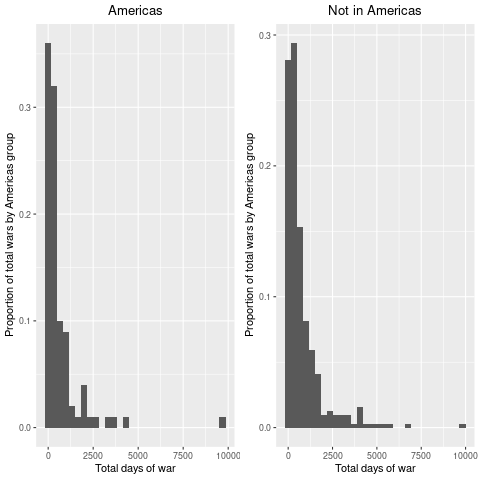
\includegraphics[width=6.67in]{/home/rstudio/Overall_plots/plot_files/Exposure_time2}

\#Battle deaths by the Americas The below shows the distribution of
deaths in the number of deaths by war type and Americas status. For the
most part they look balanced. It should be noted that an upper limit of
50000 deaths was created in order to account for plot interpretability
and to account for several wars with total deaths far greater than
50000. In the Americas group there appears to be much higher variability
in the number of deaths for wars over local issues in comparison to wars
over central control.

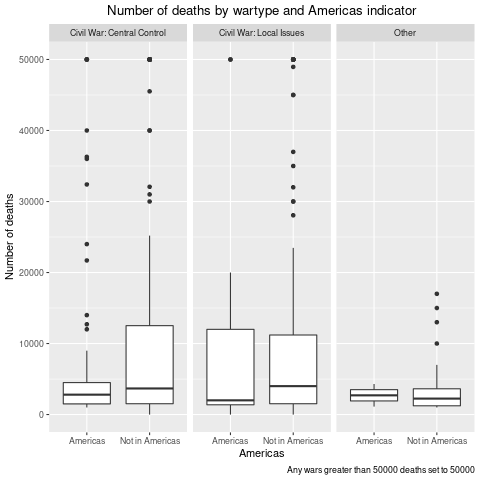
\includegraphics[width=6.67in]{/home/rstudio/Overall_plots/plot_files/Battle_deaths_Both3}

\#War type deaths Americas Adding the component of total war exposure it
was also not surprising to see large proportion of wars with lower
deaths having lower exposure time. For war type, no particular conflict
type stood-out but proportionally, the not in Americas group has a
larger variability in exposure time/deaths than wars in the the Americas
which tended to cluster more on average in the lower quadrant.

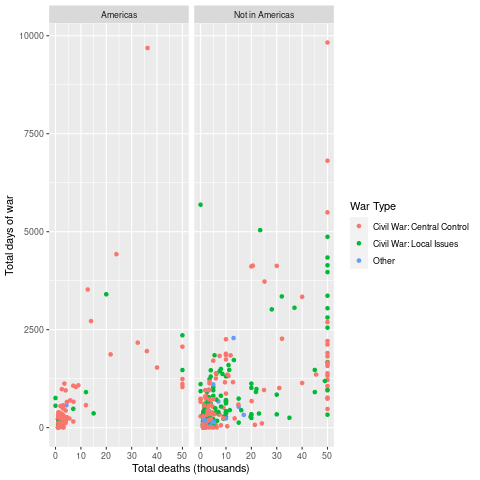
\includegraphics[width=6.67in]{/home/rstudio/Overall_plots/plot_files/War_type_deaths_Americas_4}

\#Start year A plot looking at deaths based on war start year. From
1900s onwards the civil war for central control seemed to be most
prevalent in the Americas while diversity of war type was prevalent
across the 200 year period in the non-Americas group. As mentioned in
the time to curation in table 1, the not in americas conflicts appear to
have a considerable more set of curated conflicts in the latter half of
the 20th century relative to conflicts in the Americas. Maybe one
opinion is the military hegemony in this hemisphere by the United States
to sort of dominate a lot of conflict for this hemisphere post WW-II in
comparison to the rest of the world. There does not appear to be a
linearly increasing or decreasing trend in deaths based on time of war
and war conflict in either group.

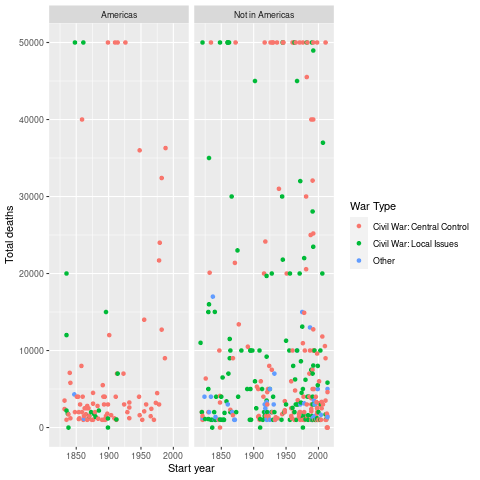
\includegraphics[width=6.67in]{/home/rstudio/Overall_plots/plot_files/Start_year_5}

\#Absolute difference in deaths Defined as the initiator
deaths-recipient deaths, once several influential points (not outliers)
were removed one can see a large proportion of initiator deaths more in
the negatives from the 1900s onwards in the not in Americas group. Maybe
this relates to some sort of potential increased ability in war
recipients being able to foresee or address conflict. Maybe it could be
greater familiarity with a `home' area in response somehow.

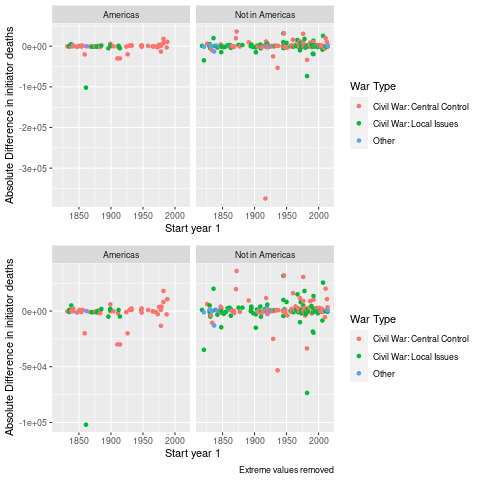
\includegraphics[width=6.67in]{/home/rstudio/Overall_plots/plot_files/Abs_6}

\#Relative difference in deaths This metric was more complicated defined
as:abs(InitiatorDeaths-RecipientDeaths)/max(abs(RecipientDeaths),abs(InitiatorDeaths))
the initiator deaths-recipient deaths, once several influential points
(not outliers) were removed visually show a larger proportion of deaths
among the initiators from the 1900s onwards.

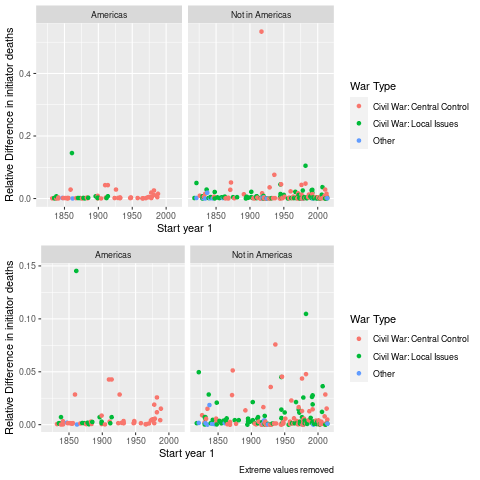
\includegraphics[width=6.67in]{/home/rstudio/Overall_plots/plot_files/Rel_7}

\#Domestic simple model Generalized linear models showing modeled the
outcome of absolute difference in deaths and then relative difference in
deaths by the Americas variable, starting year, days of exposure, and
war type. In both model sets only an association was seen with days of
exposure and relative increase in initiator deaths.

\begin{verbatim}
##                                 Description                       Variables
## 1 Absolute difference in deaths non-imputed                     (Intercept)
## 2                                                   AmericasNot in Americas
## 3                                                              StartYR_Norm
## 4                                                                WDuratDays
## 5                                           WarTypeDCivil War: Local Issues
## 6                                                             WarTypeDOther
##   Estimate Std err p-val
## 1 -5418.86 4788.97  0.26
## 2  -301.57 4421.93  0.95
## 3    28.39      34  0.40
## 4    -0.26    1.69  0.88
## 5  1414.91  3918.2  0.72
## 6  2748.99 7400.78  0.71
\end{verbatim}

\begin{verbatim}
##                                 Description                       Variables
## 1 Relative difference in deaths non-imputed                     (Intercept)
## 2                                                   AmericasNot in Americas
## 3                                                              StartYR_Norm
## 4                                                                WDuratDays
## 5                                           WarTypeDCivil War: Local Issues
## 6                                                             WarTypeDOther
##   Estimate Std err  p-val
## 1    0.008   0.006 0.1996
## 2    0.006   0.006 0.3192
## 3        0       0 0.2934
## 4        0       0 0.0048
## 5   -0.005   0.005 0.3882
## 6   -0.009    0.01 0.3520
\end{verbatim}

\#Domestic prediction non-imputed model A training and testing set
(evenly split) using 5 fold cross-validation was done. Generalized
linear models showing modeled the outcome of absolute difference in
deaths and then relative difference in deaths by the Americas variable,
starting year, days of exposure, and war type. In both model sets only
the Americas versus non-Americas showed an association in the number of
initiator deaths relative to the recipient. The prediction in the given
test set, however, R2=.008, was very low. Also an association was seen
with days of exposure and relative increase in initiator deaths.

\begin{verbatim}
##                                 Description    R2
## 1 Absolute difference in deaths non-imputed 0.009
## 2                                                
## 3                                                
## 4                                                
## 5                                                
## 6                                                
##                           Variables Estimate Std err p-val
## 1                       (Intercept) -4474.31 2944.33 0.131
## 2         `AmericasNot in Americas`  5415.25 2643.04 0.042
## 3                      StartYR_Norm    17.86   19.79 0.368
## 4                        WDuratDays    -0.58    1.11 0.600
## 5 `WarTypeDCivil War: Local Issues` -3528.15 2289.06 0.125
## 6                     WarTypeDOther -1293.59 4467.17 0.773
\end{verbatim}

\begin{verbatim}
##                                 Description    R2
## 1 Relative difference in deaths non-imputed 0.004
## 2                                                
## 3                                                
## 4                                                
## 5                                                
## 6                                                
##                           Variables Estimate Std err  p-val
## 1                       (Intercept)   0.0045  0.0034   0.20
## 2         `AmericasNot in Americas`  -0.0029  0.0031   0.34
## 3                      StartYR_Norm -1.7e-05 2.3e-05   0.47
## 4                        WDuratDays  8.1e-06 1.3e-06 <0.001
## 5 `WarTypeDCivil War: Local Issues`   0.0036  0.0027   0.18
## 6                     WarTypeDOther  -0.0019  0.0052   0.71
\end{verbatim}

\#Models deaths here The common theme across models was prediction was
very low between training and test sets. An association, however, was
seen in the war type (`local issues'). Date was re-checked and while
certainty of curation seems reasonable (some wars simply were relatively
more brutal than others), a prediction check of the imputed deaths while
removing the most extreme war (375000 death difference), showed a slight
gain in prediction (not shown but R2=.013 in comparison to .002)

\begin{verbatim}
##                             Description R2                         Variables
## 1 Absolute difference in deaths imputed  0                       (Intercept)
## 2                                                  `AmericasNot in Americas`
## 3                                                               StartYR_Norm
## 4                                                                 WDuratDays
## 5                                          `WarTypeDCivil War: Local Issues`
## 6                                                              WarTypeDOther
##   Estimate Std err p-val
## 1 -1431.34 2027.77 0.481
## 2  1459.95 2100.22 0.488
## 3    10.91   14.67 0.458
## 4    -0.06    0.64 0.924
## 5 -3257.25 1832.45 0.077
## 6  1377.77 2747.23 0.617
\end{verbatim}

\begin{verbatim}
##                             Description    R2                         Variables
## 1 Relative difference in deaths imputed 0.013                       (Intercept)
## 2                                                     `AmericasNot in Americas`
## 3                                                                  StartYR_Norm
## 4                                                                    WDuratDays
## 5                                             `WarTypeDCivil War: Local Issues`
## 6                                                                 WarTypeDOther
##   Estimate Std err  p-val
## 1   0.0045  0.0024 0.0634
## 2   0.0036  0.0025 0.1465
## 3  1.6e-06 1.7e-05 0.9278
## 4  2.3e-06 7.6e-07 0.0024
## 5 -0.00024  0.0022 0.9135
## 6  -0.0031  0.0033 0.3442
\end{verbatim}

\#Internationalized Non-imputed

Network

\begin{verbatim}
##                                      Description    R2
## 1 Intl Absolute difference in deaths non-imputed 0.011
## 2                                                     
## 3                                                     
## 4                                                     
## 5                                                     
## 6                                                     
## 7                                                     
## 8                                                     
##                          Covariates Estimate Std err p-val
## 1                       (Intercept)  -2875.7 2354.04 0.224
## 2         `AmericasNot in Americas`  3177.52 2265.41 0.163
## 3                      StartYR_Norm    15.32   16.08 0.342
## 4                        WDuratDays     -2.2    0.98 0.027
## 5 `WarTypeDCivil War: Local Issues` -2670.35 1858.04 0.153
## 6                     WarTypeDOther -1991.32 3945.77 0.614
## 7                   InitiatorForces        0       0 0.856
## 8                   RecipientForces        0       0 0.067
\end{verbatim}

\begin{verbatim}
##                                      Description    R2
## 1 Intl Relative difference in deaths non-imputed 0.033
## 2                                                     
## 3                                                     
## 4                                                     
## 5                                                     
## 6                                                     
## 7                                                     
## 8                                                     
##                          Covariates Estimate Std err  p-val
## 1                       (Intercept)   -0.011   0.016 0.4647
## 2         `AmericasNot in Americas`  0.00013   0.013 0.9915
## 3                      StartYR_Norm  3.1e-05 0.00014 0.8263
## 4                        WDuratDays  3.4e-05   1e-05 <0.001
## 5 `WarTypeDCivil War: Local Issues`  -0.0037   0.012 0.7478
## 6                     WarTypeDOther  0.00079   0.025 0.9744
## 7                   InitiatorForces  8.1e-09 1.9e-08 0.6738
## 8                   RecipientForces  9.1e-09 2.8e-09 0.0013
\end{verbatim}

\#Internationalized Imputed Network

\begin{verbatim}
##                                      Description    R2
## 1 Intl Absolute difference in deaths non-imputed 0.011
## 2                                                     
## 3                                                     
## 4                                                     
## 5                                                     
## 6                                                     
## 7                                                     
## 8                                                     
##                          Covariates Estimate Std err p-val
## 1                       (Intercept)  -2875.7 2354.04 0.224
## 2         `AmericasNot in Americas`  3177.52 2265.41 0.163
## 3                      StartYR_Norm    15.32   16.08 0.342
## 4                        WDuratDays     -2.2    0.98 0.027
## 5 `WarTypeDCivil War: Local Issues` -2670.35 1858.04 0.153
## 6                     WarTypeDOther -1991.32 3945.77 0.614
## 7                   InitiatorForces        0       0 0.856
## 8                   RecipientForces        0       0 0.067
\end{verbatim}

\begin{verbatim}
##                                      Description    R2
## 1 Intl Relative difference in deaths non-imputed 0.033
## 2                                                     
## 3                                                     
## 4                                                     
## 5                                                     
## 6                                                     
## 7                                                     
## 8                                                     
##                          Covariates Estimate Std err  p-val
## 1                       (Intercept)   -0.011   0.016 0.4647
## 2         `AmericasNot in Americas`  0.00013   0.013 0.9915
## 3                      StartYR_Norm  3.1e-05 0.00014 0.8263
## 4                        WDuratDays  3.4e-05   1e-05 <0.001
## 5 `WarTypeDCivil War: Local Issues`  -0.0037   0.012 0.7478
## 6                     WarTypeDOther  0.00079   0.025 0.9744
## 7                   InitiatorForces  8.1e-09 1.9e-08 0.6738
## 8                   RecipientForces  9.1e-09 2.8e-09 0.0013
\end{verbatim}

\#Overall clustering Aim 3 was multi-fold: to cluster wartype, the
Americas indicator variable, time since war started since 1814
basically, whether the war was internationalized, duration of exposure
(days), initiator deaths, recipient deaths, and relative difference in
deaths. A distance metric for mixed data types (Gower) was used and
clustering via KMeans. tSNE plots showed the segmentation of the
variability of the gower's distance metric, and the clusters were
visually plotted.

Below shows the top 2 TSNE dimensions by cluster and showing distinct
separation throughout.

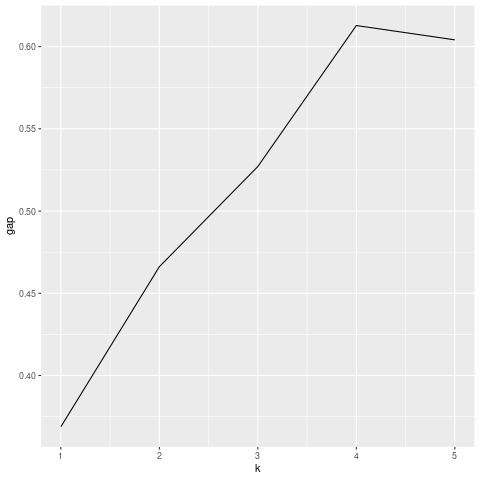
\includegraphics[width=6.67in]{/home/rstudio/Overall_plots/plot_files/Gap_stat}
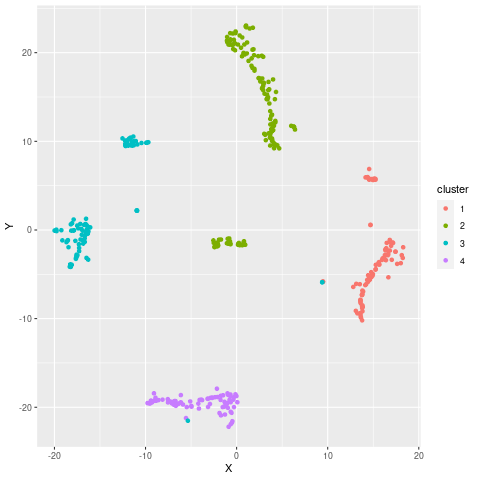
\includegraphics[width=6.67in]{/home/rstudio/Aim2_out_clustering/Cluster_Files/Aim2_TSNE}

\#Overall clustering by variables

As described above the four clusters showed a distince pattern across
the variables in their construction. Clearly defined Americas (cluster
1), and non-Americas clusters were shown (2 through 4) which looked very
interesting albeit a little fishy. The largest proportion of those where
the recipient won was in the Americas cluster. Otherwise stalemates,
compromises, etc. were the largest in all three of the specific
clusters. Cluster 3 could be established as the highest difference in
deaths for the initiator for some reason. Cluster 3 could also be seen
to have the most modern (time since curation of 1814) conflict cluster
with an average starting time of conflicts ranging from the late 1950s.

\begin{verbatim}
## 
## --------Summary descriptives table by 'cluster'---------
## 
## ______________________________________________________________________________________________________ 
##                                               1                2               3               4       
##                                              N=98            N=147            N=92           N=83      
## ¯¯¯¯¯¯¯¯¯¯¯¯¯¯¯¯¯¯¯¯¯¯¯¯¯¯¯¯¯¯¯¯¯¯¯¯¯¯¯¯¯¯¯¯¯¯¯¯¯¯¯¯¯¯¯¯¯¯¯¯¯¯¯¯¯¯¯¯¯¯¯¯¯¯¯¯¯¯¯¯¯¯¯¯¯¯¯¯¯¯¯¯¯¯¯¯¯¯¯¯¯¯ 
## Americas:                                                                                              
##     Americas                              98 (100%)        0 (0.00%)       2 (2.17%)       0 (0.00%)   
##     Not in Americas                       0 (0.00%)       147 (100%)       90 (97.8%)      83 (100%)   
## OutcomeE:                                                                                              
##     Initiator Won                         10 (10.2%)      28 (19.0%)       4 (4.35%)      12 (14.5%)   
##     Other                                 59 (60.2%)      115 (78.2%)      78 (84.8%)     57 (68.7%)   
##     Recipient Won                         29 (29.6%)       4 (2.72%)       10 (10.9%)     14 (16.9%)   
## WarTypeC:                                                                                              
##     Civil War: Central Control            79 (80.6%)       0 (0.00%)       61 (66.3%)      83 (100%)   
##     Civil War: Local Issues               17 (17.3%)      111 (75.5%)      27 (29.3%)      0 (0.00%)   
##     Intercommunal                         0 (0.00%)       26 (17.7%)       2 (2.17%)       0 (0.00%)   
##     Regional Internal                     2 (2.04%)       10 (6.80%)       2 (2.17%)       0 (0.00%)   
## WDuratDays                                665 (1226)      674 (1041)      1073 (1450)      641 (880)   
## InitiatorDeaths                          6589 (27942)     3267 (9287)    17903 (72554)   5558 (22675)  
## RecipientDeaths                          8304 (38846)    3327 (13458)    21608 (97358)   4945 (23164)  
## RelDiffDeaths                            0.01 (0.02)      0.01 (0.01)     0.02 (0.08)     0.01 (0.01)  
## AbsDiffDeaths                          -2850.22 (15214) -121.26 (10905) -7100.94 (55926)  942 (8592)   
## StartYR_Norm                             75.2 (43.3)      102 (60.5)       143 (50.3)     129 (51.5)   
## OutcomeC:                                                                                              
##     Compromise                            3 (3.06%)       16 (10.9%)       15 (16.3%)      5 (6.02%)   
##     Conflict continues below war level    1 (1.02%)       13 (8.84%)       4 (4.35%)       7 (8.43%)   
##     Side A wins                           60 (61.2%)      77 (52.4%)       32 (34.8%)     43 (51.8%)   
##     Side B wins                           32 (32.7%)      14 (9.52%)       20 (21.7%)     19 (22.9%)   
##     Stalemate                             0 (0.00%)       14 (9.52%)       5 (5.43%)       4 (4.82%)   
##     War ongoing as of end of 2014         1 (1.02%)        1 (0.68%)       7 (7.61%)       3 (3.61%)   
##     War transformed into another War      1 (1.02%)       12 (8.16%)       9 (9.78%)       2 (2.41%)   
## TotalBDeaths                            17320 (66971)    11898 (29275)   50105 (167912)  13853 (45569) 
## Intnl                                    0.03 (0.17)      0.00 (0.00)     0.99 (0.10)     0.00 (0.00)  
## ¯¯¯¯¯¯¯¯¯¯¯¯¯¯¯¯¯¯¯¯¯¯¯¯¯¯¯¯¯¯¯¯¯¯¯¯¯¯¯¯¯¯¯¯¯¯¯¯¯¯¯¯¯¯¯¯¯¯¯¯¯¯¯¯¯¯¯¯¯¯¯¯¯¯¯¯¯¯¯¯¯¯¯¯¯¯¯¯¯¯¯¯¯¯¯¯¯¯¯¯¯¯
\end{verbatim}

\#Aim 4 network composition While not much was shown, several network
plots were constructed. A walk trap community search algorithm was
implemented and is generally a solid approach when not much is known
about the given network structure. Weights between conflicts were
normalized differences in conflicts and directed graph structure was
created representing initiator to recipient relationships.

The first overall network plot shows all the wars together and their
post memberships. Roughly a 100 communities were found, and rather than
pruning, the second plot shows the distribution of community membership
by wars representing the largest communities. The third plot shows the
communities consolidated by the first three most prevalent communities
and the fourth determined as `other'. Edge attributes explaining these 3
particular communities will be evaluated as a next-to-do.\\

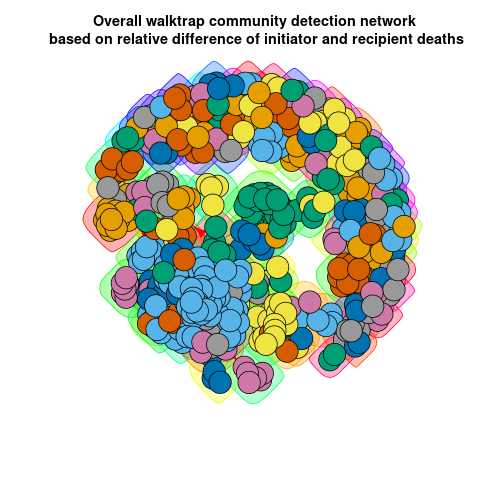
\includegraphics[width=6.67in]{/home/rstudio/Networks/Network_Files/Ov}
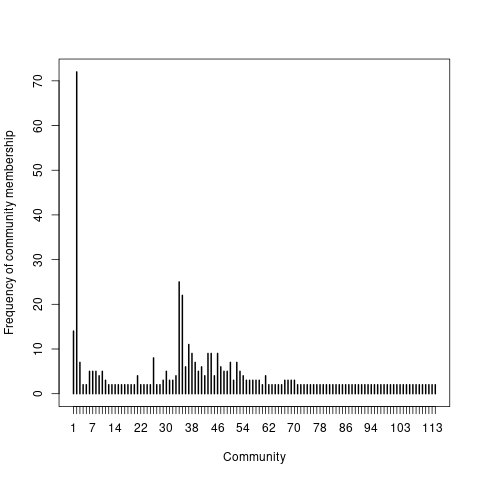
\includegraphics[width=6.67in]{/home/rstudio/Networks/Network_Files/Membership}
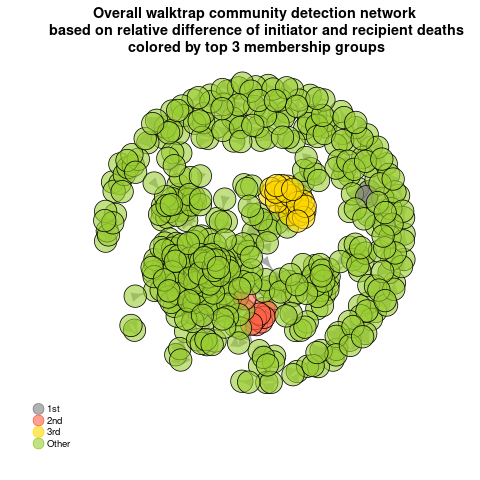
\includegraphics[width=6.67in]{/home/rstudio/Networks/Network_Files/Membership_consolidated}

\#Conclusions

Descriptive plots showed some interesting patterns such as considerably
less conflicts post WW-2 in the hemisphere occupied by North and South
America relative to the rest of the world.\\

The most interesting part of the project turned out to be the initial
clustering and descriptive representation with the key war variables and
in particular the Americas variable. Prediction modeling initially
wanted to look at sub groups or tree based models after the GLMs. But
such low performance and variability in the differences in initiator and
recipient deaths probably contributed to the poor performance. Rather
than exploring the tree models, a mixed data clustering approach looked
at the key war variables and generated some interesting results

Another initial aim to look at data-driven eras or model-based
clustering as well as waves of a given war. Unfortunately the date
curation for many waves beyond the first wave was more sparse than
originally thought, and looking at time based eras did not have the same
interest. Finally, the network community structure work found several
clusters of communities but analysis is still in process. Other
approaches could be considered that also try to look at the
relationships in a flow of relationships.

\end{document}
